\documentclass{standalone}
\usepackage{tikz}
\begin{document}

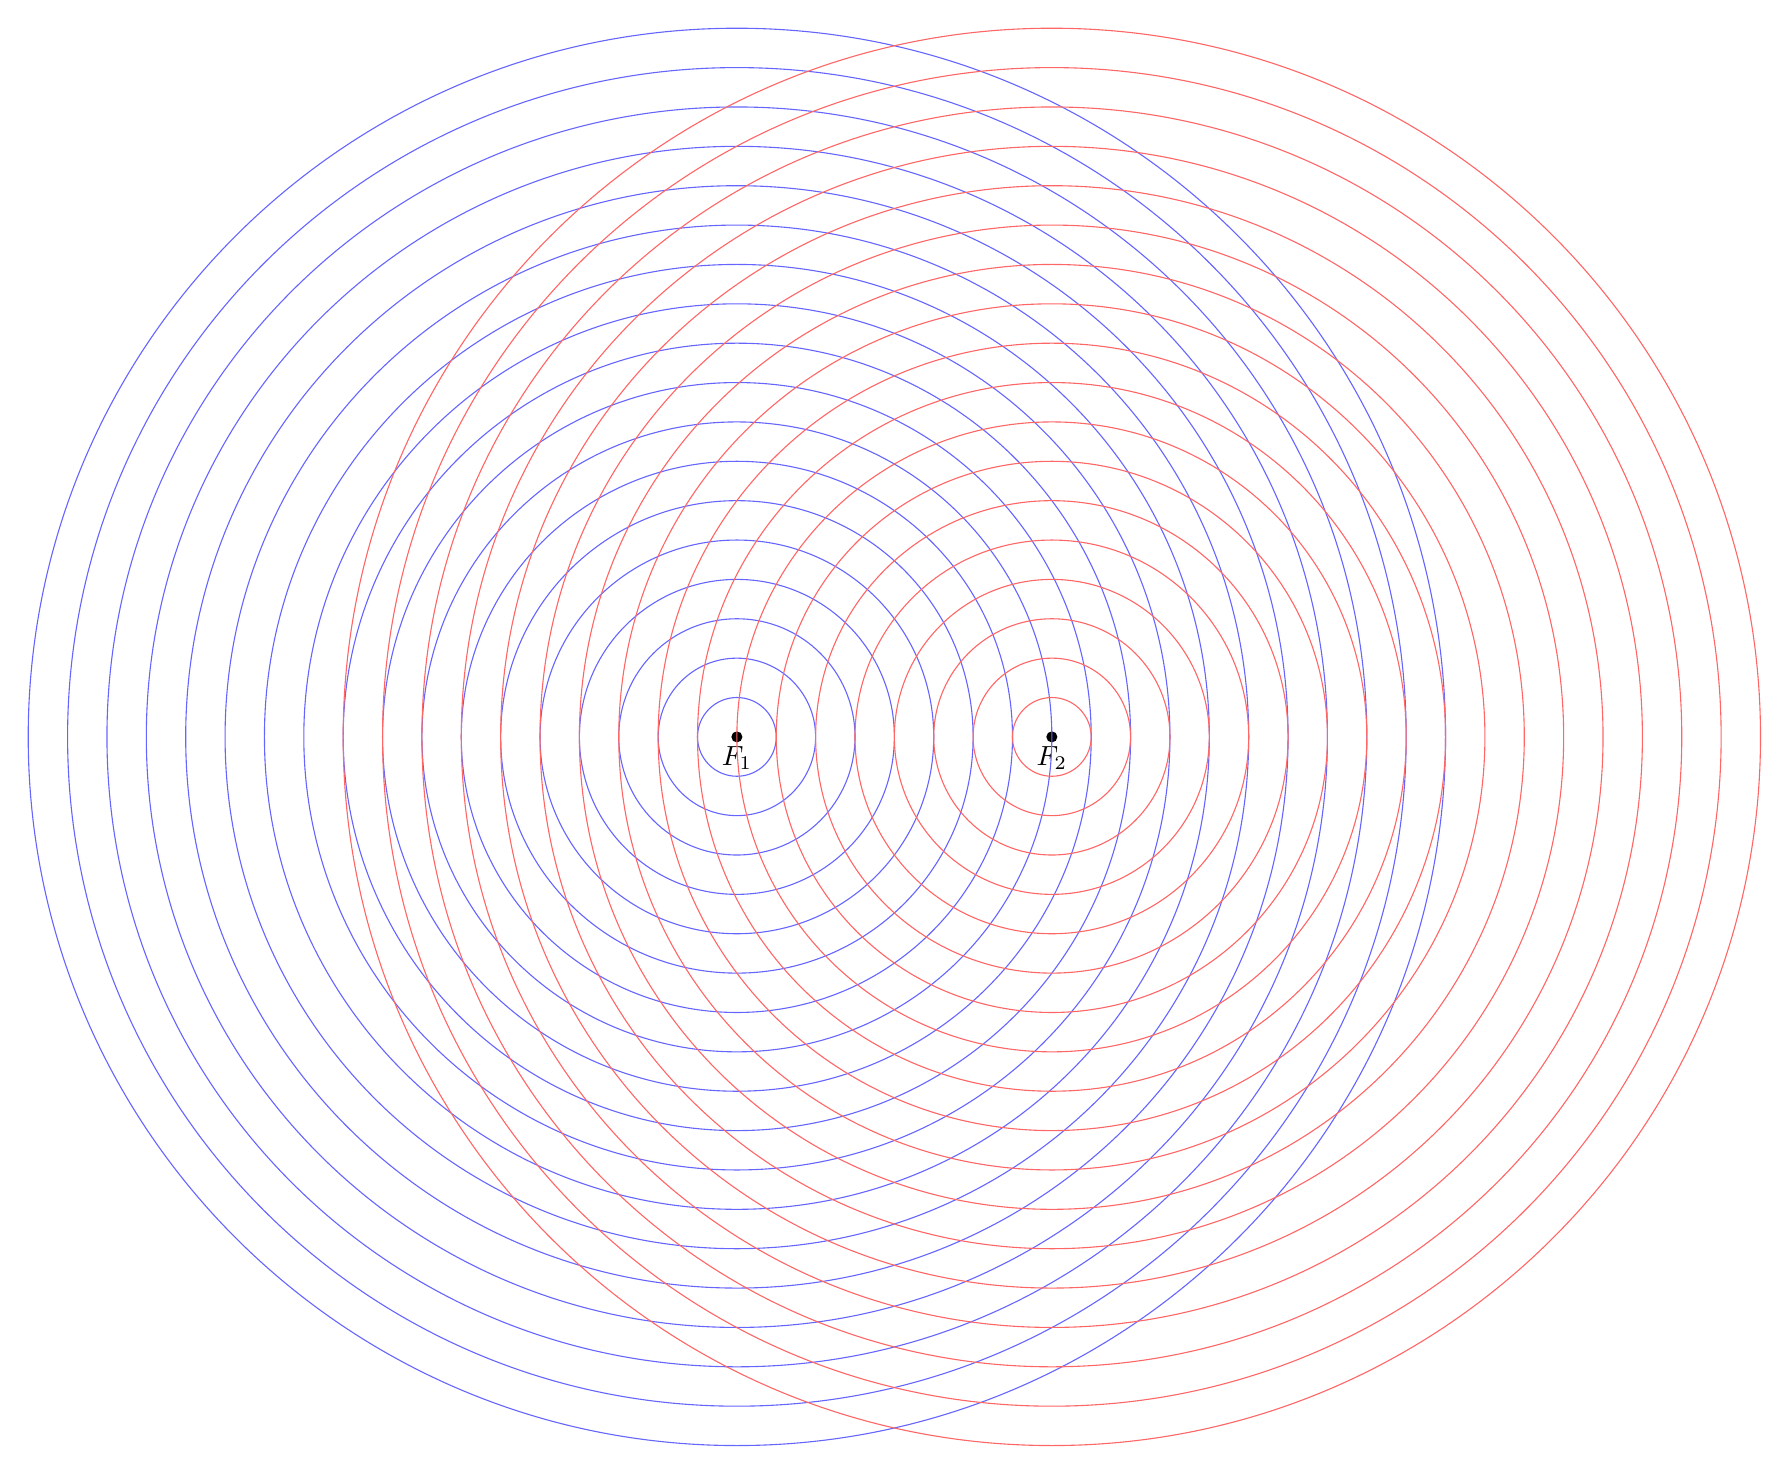
\begin{tikzpicture}[scale=1]

% Points F1 and F2
\coordinate (F1) at (-2,0);
\coordinate (F2) at (2,0);

% Draw the points
\fill (F1) circle (2pt) node[below] {$F_1$};
\fill (F2) circle (2pt) node[below] {$F_2$};

% Circles centered at F1
\foreach \r in {1,2,...,18}
{
    \draw[blue!60] (F1) circle (\r*0.5);
}

% Circles centered at F2
\foreach \r in {1,2,...,18}
{
    \draw[red!60] (F2) circle (\r*0.5);
}

\end{tikzpicture}
\end{document}